\documentclass[10pt,a4paper]{article}
\usepackage[margin=2.5cm]{geometry}
\usepackage[english]{babel}
\usepackage[colorlinks=true, allcolors=blue]{hyperref}
\usepackage{minted}
\usepackage{natbib}
\setcitestyle{authoryear,open={(},close={)}}
\usepackage{amsmath}
\usepackage{amssymb}
\usepackage{amsfonts}
\usepackage{multicol}
\usepackage{listings}
\usepackage{gensymb}
\usepackage{wrapfig}
\usepackage{graphicx}
\usepackage{fontspec}
\usepackage{tabularx}
\usepackage{amsfonts}
\usepackage{xcolor}
\usepackage{graphicx}
\usepackage{fancyhdr}
\usepackage{subcaption}

\graphicspath{ {./images/} }

\pagestyle{fancy}
\fancyhead{}
\renewcommand{\headrulewidth}{0pt}
\fancyfoot[L]{\footnotesize{George Hester (201124124) - COMP3011}}
\fancyfoot[R]{\footnotesize{\thepage}}
\fancyfoot[C]{}
% \fancyfoot[C]{\includegraphics[height=8pt]{vulpz.png}}

\renewcommand{\thesection}{\arabic{section}}
% \setmonofont{Berkeley Mono Trial}
% \setmainfont{Libre Baskerville}
% \setmainfont{Monaspace Neon Light}
% \setmainfont{Euclid Circular B}
\setmainfont{TX-02 Retina}
\setmonofont{TX-02 Bold}
\usemintedstyle{vulpz}

\begin{document}

\noindent
\Huge
\textbf{Train API}
\normalsize
\noindent
\newline
\newline
Updated - 10-03-2026

\tableofcontents

\newpage
\section{Resource Links}

\begin{itemize}
  \item \href{https://github.com/georgehester/train-api}{GitHub Repository}
  \item \href{http://documentation.api.train.vulpz.com}{Documentation}
  \item \href{https://docs.google.com/presentation/d/1i460dvt5QaJjt-JxWjruQaugBEQW9677Q9r5tmAWCv4/edit?usp=sharing}{Presentation}
\end{itemize}

\section{Documentation}

Documentation is provided in a live interface rather than PDF format. The live interface can be found using the link above or \url{http://documentation.api.train.vulpz.com}. The different endpoints provided by the API are organised into categories in the navigation pane on the left. Each endpoint has schema definitions for its possible requests and responses. All the models representing request and response types are under the Models heading on the navigation panel and can be expanded to show their child components.

\section{Data Collection / Manipulation}

Due to my choice of data set I found that Generative AI would struggle with understanding and parsing it. This is likely because the data is provided by real systems that have complicated interfaces and schema types. Along with this the documentation for these systems is quite hidden and would not have been included in the models training set giving it no reference points of how to understand the formats presented.

\noindent
\newline
The data was collected from a number of data sources provided by NRE (National Rail) and NWR (Network Rail) through the RDM (Rail Data Marketplace). The following resources were heavily utilised.

\begin{itemize}
  \item Network Rail Corpus
  \item Network Rail Schedule
  \item National Rail Knowledge Base Stations
  \item National Rail Darwin Push Port (Archive Provided By David Wheatley)
  \item National Rail Darwin Timetable
\end{itemize}

\noindent
Once the data was collected in its respective formats summing to ~100GB python scripts provided in the \texttt{collection} folder are used to generate the SQL database needed for the API.

\noindent
\newline
The first operation that must be undertook is the creation of the \texttt{stations} table. This can be done by running the Python module with the following command.

\noindent
\newline
\texttt{python -m collection.stations.generate}

\noindent
\newline
This command will generate the stations table combining data from Network Rail Corpus and the National Rail Knowledge Base Stations.

\noindent
\newline
Next the timetable must be generated. The following script generates the timetable data using the National Rail Darwin Timetable for each of the stations previously populated into the database.

\noindent
\newline
\texttt{python -m collection.timetable.generate}

\noindent
\newline
Finally we have to replay the National Rail Darwin Push Port messages. The archive we use is a log of all the XML messages from Darwin, these messages must be replayed in chronological order to generate the correct database state. This is done with the final Python module.

\noindent
\newline
\texttt{python -m collection.pushport.replay}

\noindent
\newline
It would be ideal to also compile data from other source to improve the accuracy of the dataset however due to time constraints this was not possible.

\section{Architecture}

For the API a choice was made to use the Go programming language. This choice was made on the basis that Go is a compiled static typed language which allows it to be highly performant when compared to APIs defined in other interpreted programming languages such as Python or JavaScript.

\noindent
\newline
To make development of the API in Go simpler an API framework was employed. In this case the API uses a common well documented framework called Gin. This choice means there is plenty of documentation of how to use the framework and that an LLM would likely have a good amount of training data related to the framework to infer from.

\noindent
\newline
For the database a choice was made to use PostgreSQL, this choice was made after trial testing with SQLite. SQLite started to show extreme slowdown during the generation of the dataset, mainly the \texttt{stops} table, this forced the choice of technology to be reconsidered. Instead of operating as a single portable file which is programmatically controlled through a driver PostgreSQL provides a full fledged engine making it much more performant and able to handle large volumes of traffic. Along with this PostgreSQL allows for more fine grained control of data types such as the use of \texttt{VARCHAR}, reducing the overall storage usage of the database.

\section{Database Schema}

The database uses a core schema relating \texttt{customers} to \texttt{applications} and an additional table of \texttt{administrators}. Along with this there is also the tables which store the dataset, these are organised into \texttt{stations}, \texttt{journeys} and \texttt{stops}. Each station can be related to many stops and a journey can have many stops. There is also a \texttt{stations\_analysis} table which is generated during data manipulation.

\section{Authentication}

Endpoints in the API are organised into three different levels of authorisation.

\begin{itemize}
  \item Administration - Covers endpoints used by administrators to perform actions such as updating an application approval status.
  \item Protected - Covers endpoints that the customer can use to manage their account and applications, i.e. creating new applications, refreshing application keys.
  \item Product - This group covers endpoints that relate to the actual end user data API provided, authentication on these endpoints does not require login and instead makes use of a Bearer token scheme.
\end{itemize}

\noindent
Product endpoints rely on the Bearer token authorisation scheme, this means that an application key can be used by an autonomous user to make requests. This allows for the development of external applications which make use of our API. The Authorization header provided when making requests should follow the format \texttt{Bearer <base64("<applicationId>:<applicationKey>")>} \citep{bearer}, an adaptation of OAuth 2.0 Bearer authorisation \citep{rfc6750}.

\noindent
\newline
Administration endpoints make use of login endpoint which returns a JWT (JSON Web Token) \citep{rfc7519} which can be used for authorisation. The token is used on subsequent requests to the administration endpoints. Along with verifying the JWT the service also checks that the JWT claims \texttt{"type"} attribute is set to \texttt{administrator}, this allows the service to check that the given requester should have access to the administrative endpoints. The claims in the JWT are signed using the services private key so they can be verified as untampered.

\noindent
\newline
Protected endpoints make use of the same JWT (JSON Web Token) authorisation scheme but do not check the \texttt{"type"} claim. These endpoints instead verify the validity of the token then check that the customer requesting data has authorisation to access the customer data they are requesting. This is usually that the requested data is the customers own, so the identifier in the claims matches the identifier in the URL.

\noindent
\newline
To sign JWTs (JSON Web Tokens) the service uses a public private Ed25519 key pair and the EdDSA digital signature scheme. This choice was made as Ed25519 presents one of the most secure signature schemes currently adopted in wide use while still being performant for low tier hardware.

% \begin{verbatim}
% ┌────────────────────────────────┐
% │                                │
% │         Administration         │
% │                                │
% └────────────────────────────────┘
% ┌────────────────────────────────┐
% │                                │
% │           Protected            │
% │                                │
% └────────────────────────────────┘
% ┌────────────────────────────────┐
% │                                │
% │            Product             │
% │                                │
% └────────────────────────────────┘
% \end{verbatim}

\section{Testing}

Testing of the application is performed using two methodologies. The first is a set of unit tests written in Go, these unit tests can be invoked using the Go CLI or through CI on GitHub Actions when a commit is made to the repository.

\noindent
\newline
The unit tests have coverage over general portable functionality in the application rather than testing entire endpoints at once. This means that they can be run in isolation but also that they fail to cover as much of the code as would be desired. To aid in code coverage a Postman environment and a generated client interface are used to test the end-to-end functionality of each of the endpoints provided.

\section{Generative AI Declaration}

Generative AI was used to aid with the development of both the API application itself and the data manipulation scripts. The following Generative AI tools were used.

\begin{itemize}
  \item T3 Chat (\href{https://t3.chat}{t3.chat})
  \item GitHub Copilot (\href{https://github.com/features/copilot}{copilot})
\end{itemize}

\noindent
The T3 Chat tool allows usage of a wide range of LLM models in a chat interface which aided with the development of the application through prompts phrased as questions.

\noindent
\newline
GitHub Copilot integrates a chat interface into the VSCode editor and provides "Agent" mode. In this mode the models can automatically search for context within your workspace and update files. This allows for prompt to be used which ask the AI model to make changes to the code itself.

\noindent
\newline
The primary models used through these tools were Claude Sonnet 4.6 and GPT 5.3 Codex due to their high LiveBench \citep{livebench} score and balanced token cost.

% \begin{figure}[htbp]
%   \centering
%   \includegraphics[width=0.6\linewidth]{pwm.png}
%   \caption{Timed PWM repeated every 20ms}
%   \label{fig:pwm}
% \end{figure}

\newpage
\bibliographystyle{plainnat}
\nocite{rfc6750}
\bibliography{references}

\newpage
\section{Generative AI Examples}

\begin{figure}[htbp]
  \centering
  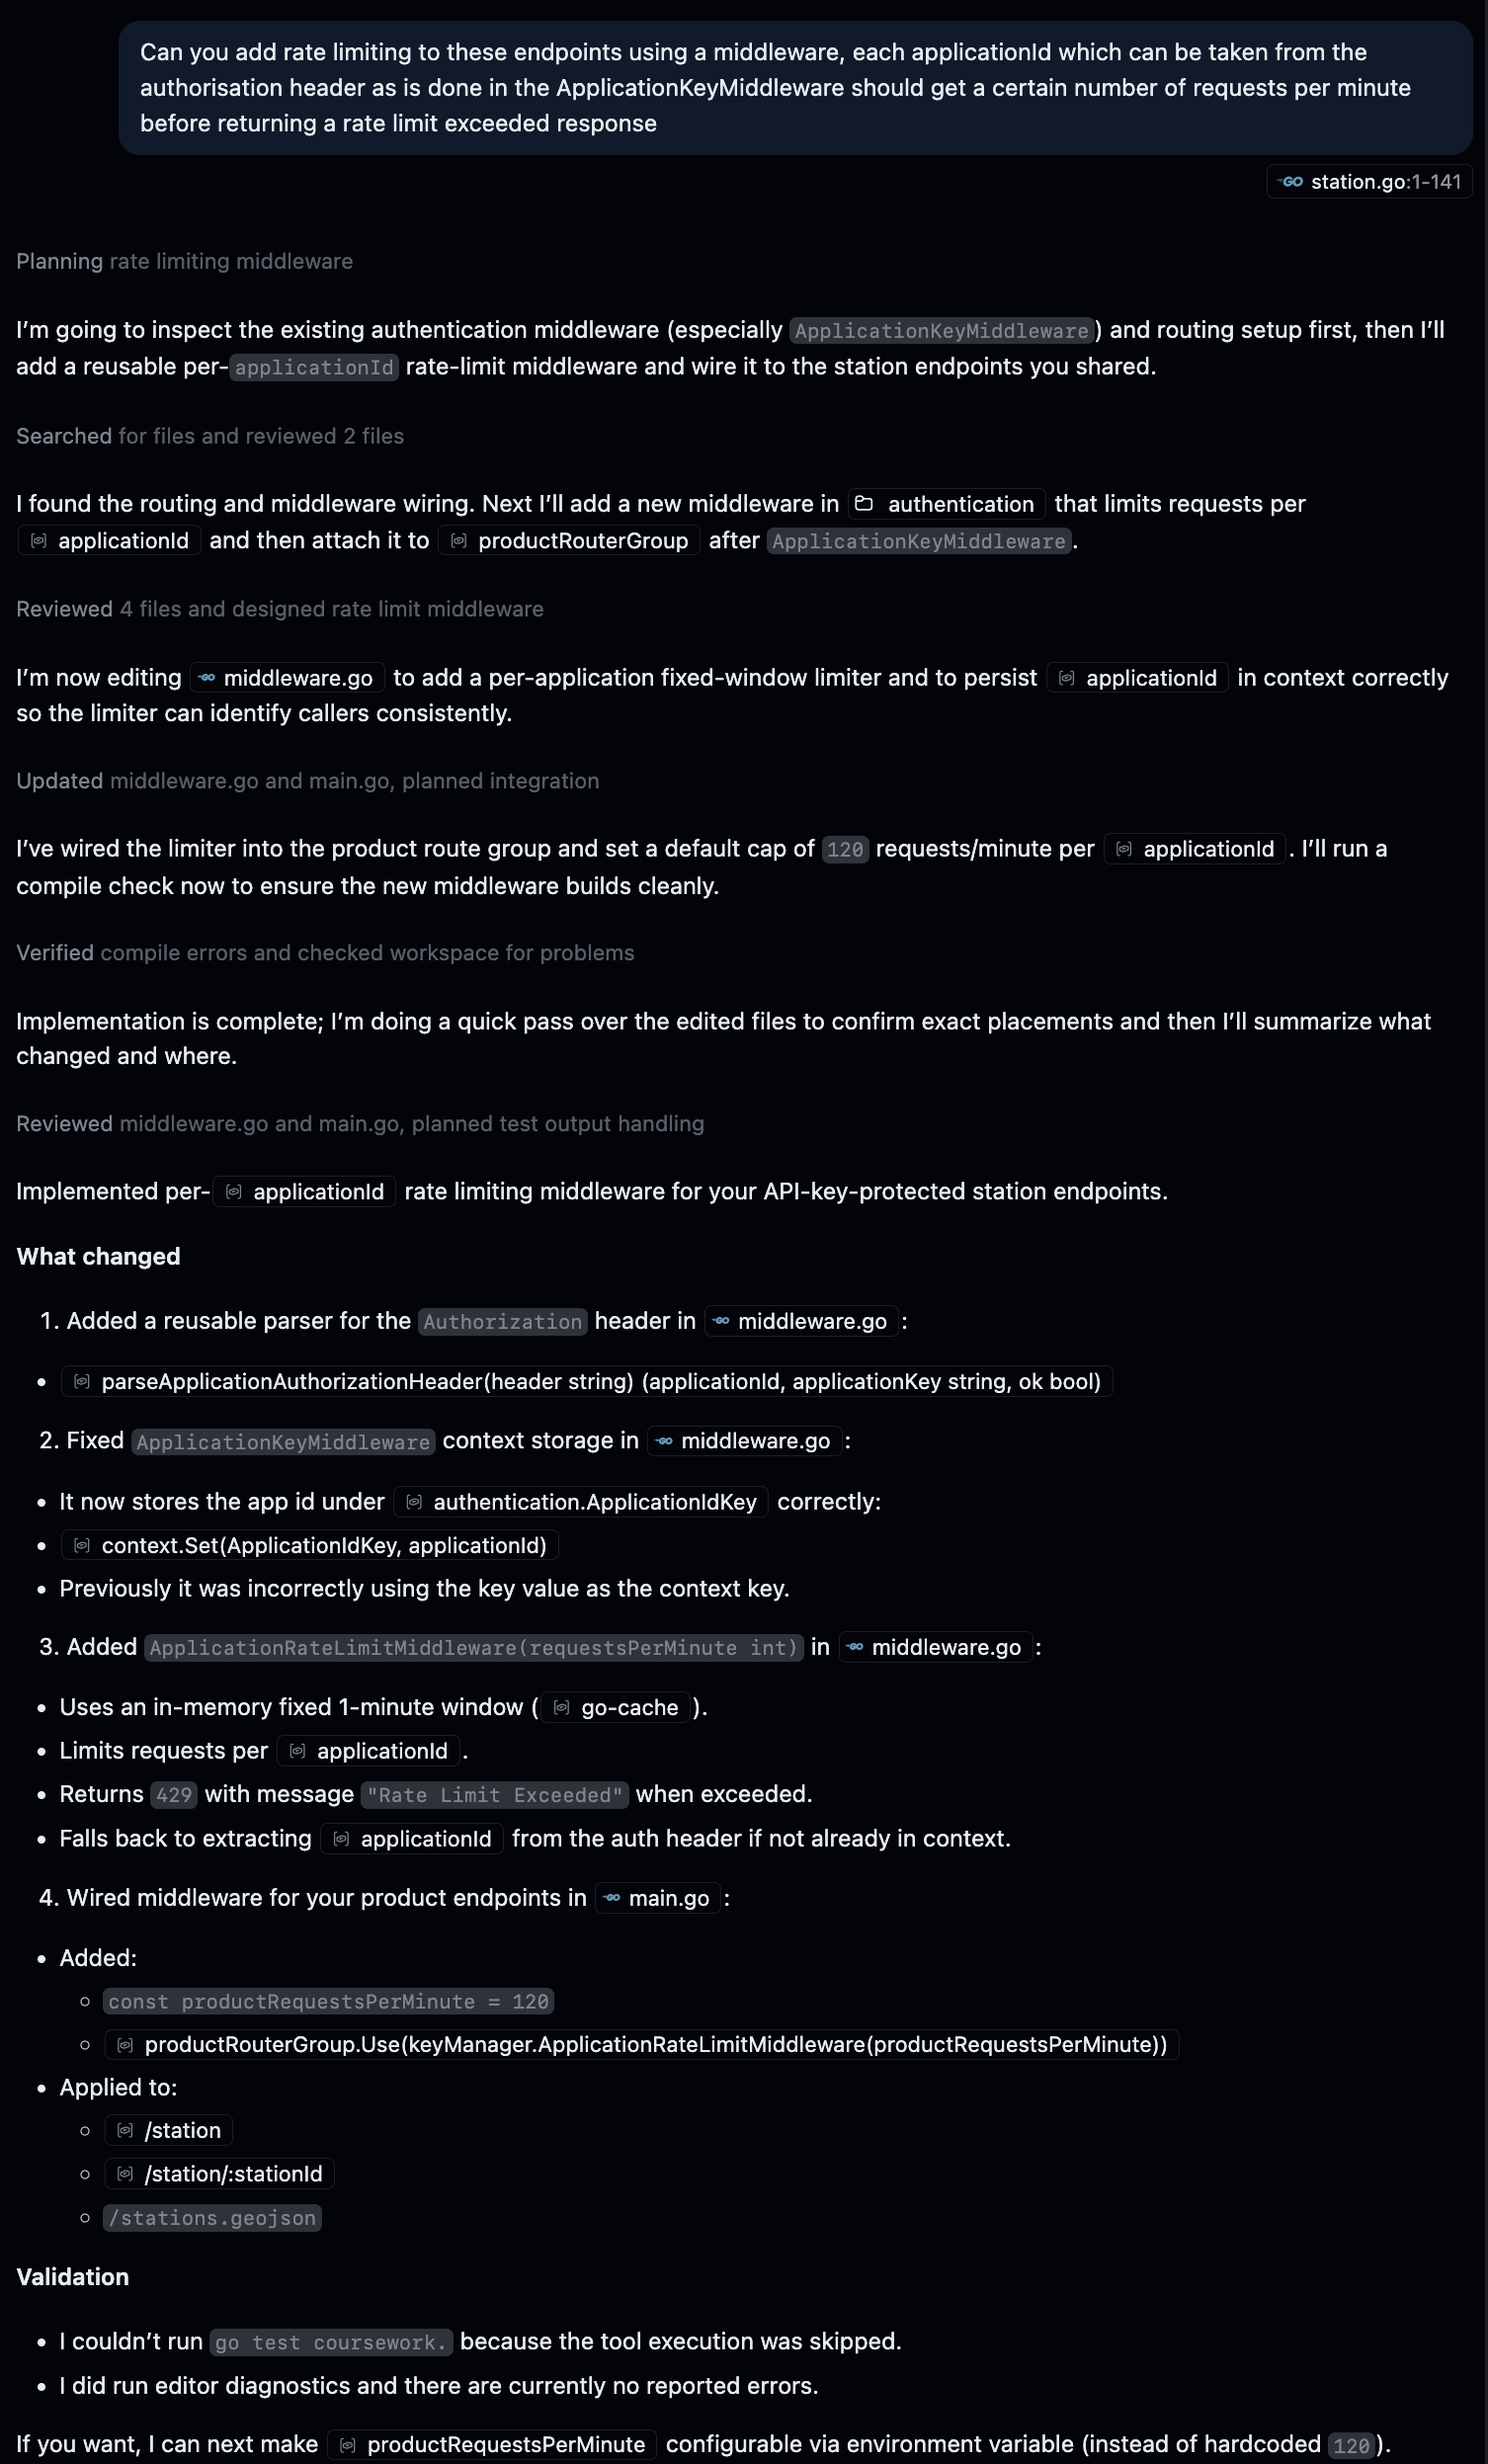
\includegraphics[width=0.6\linewidth]{ai-02.png}
\end{figure}

\begin{figure}[htbp]
  \centering
  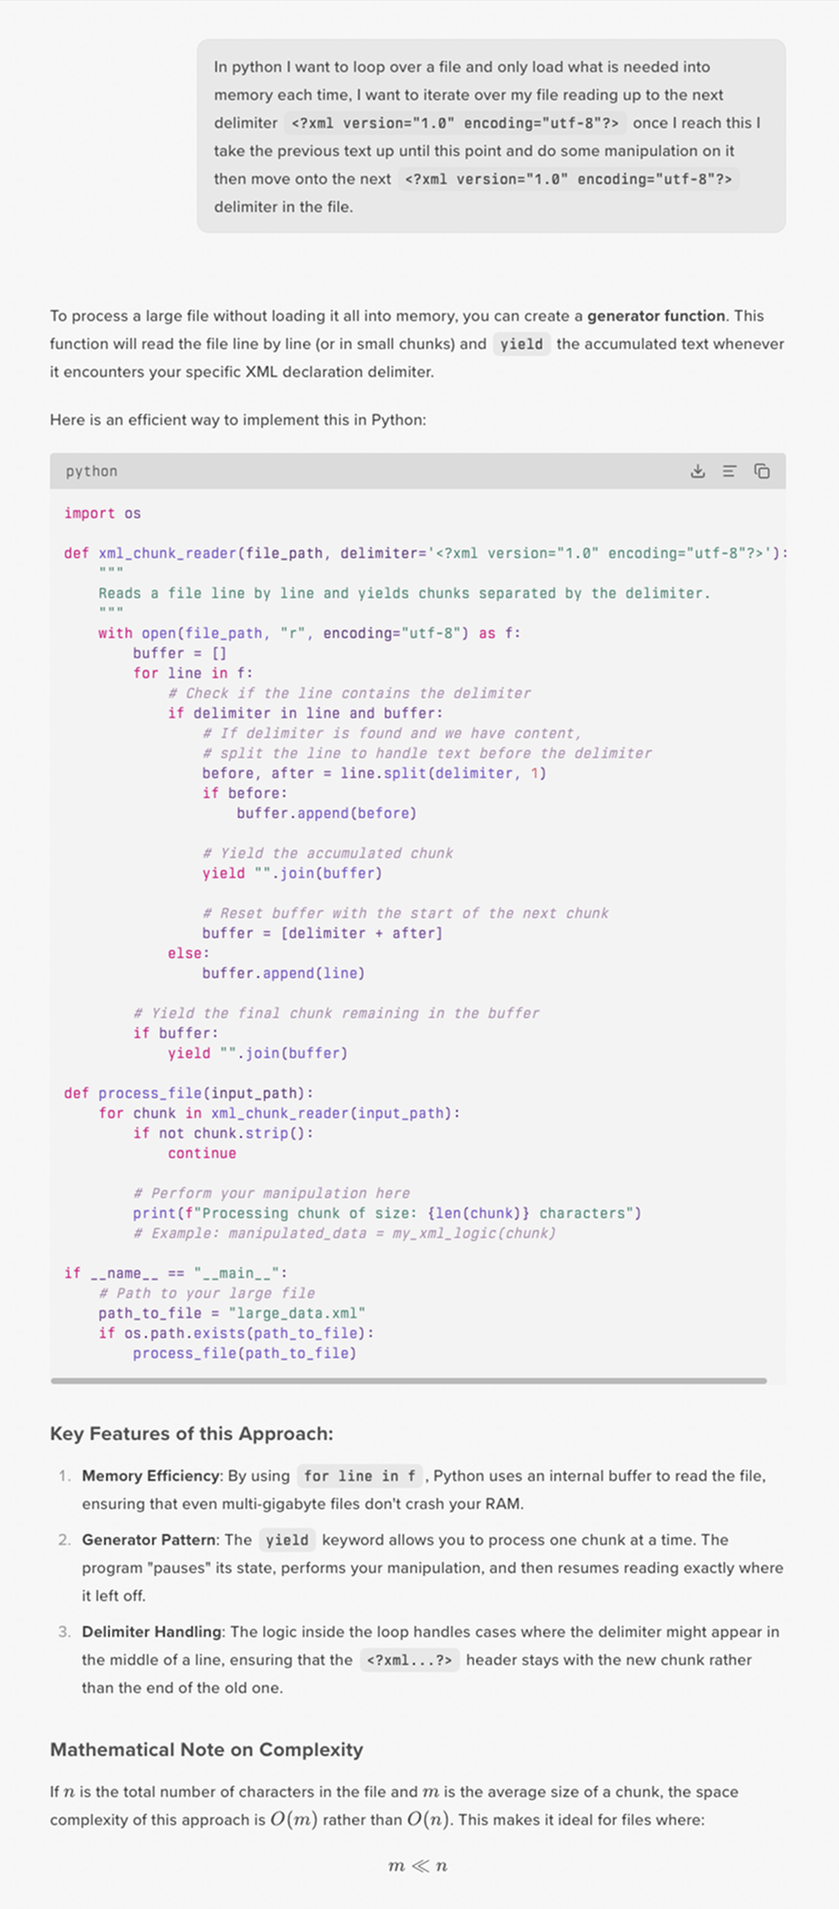
\includegraphics[width=0.6\linewidth]{ai-01.png}
\end{figure}

\begin{figure}[htbp]
  \centering
  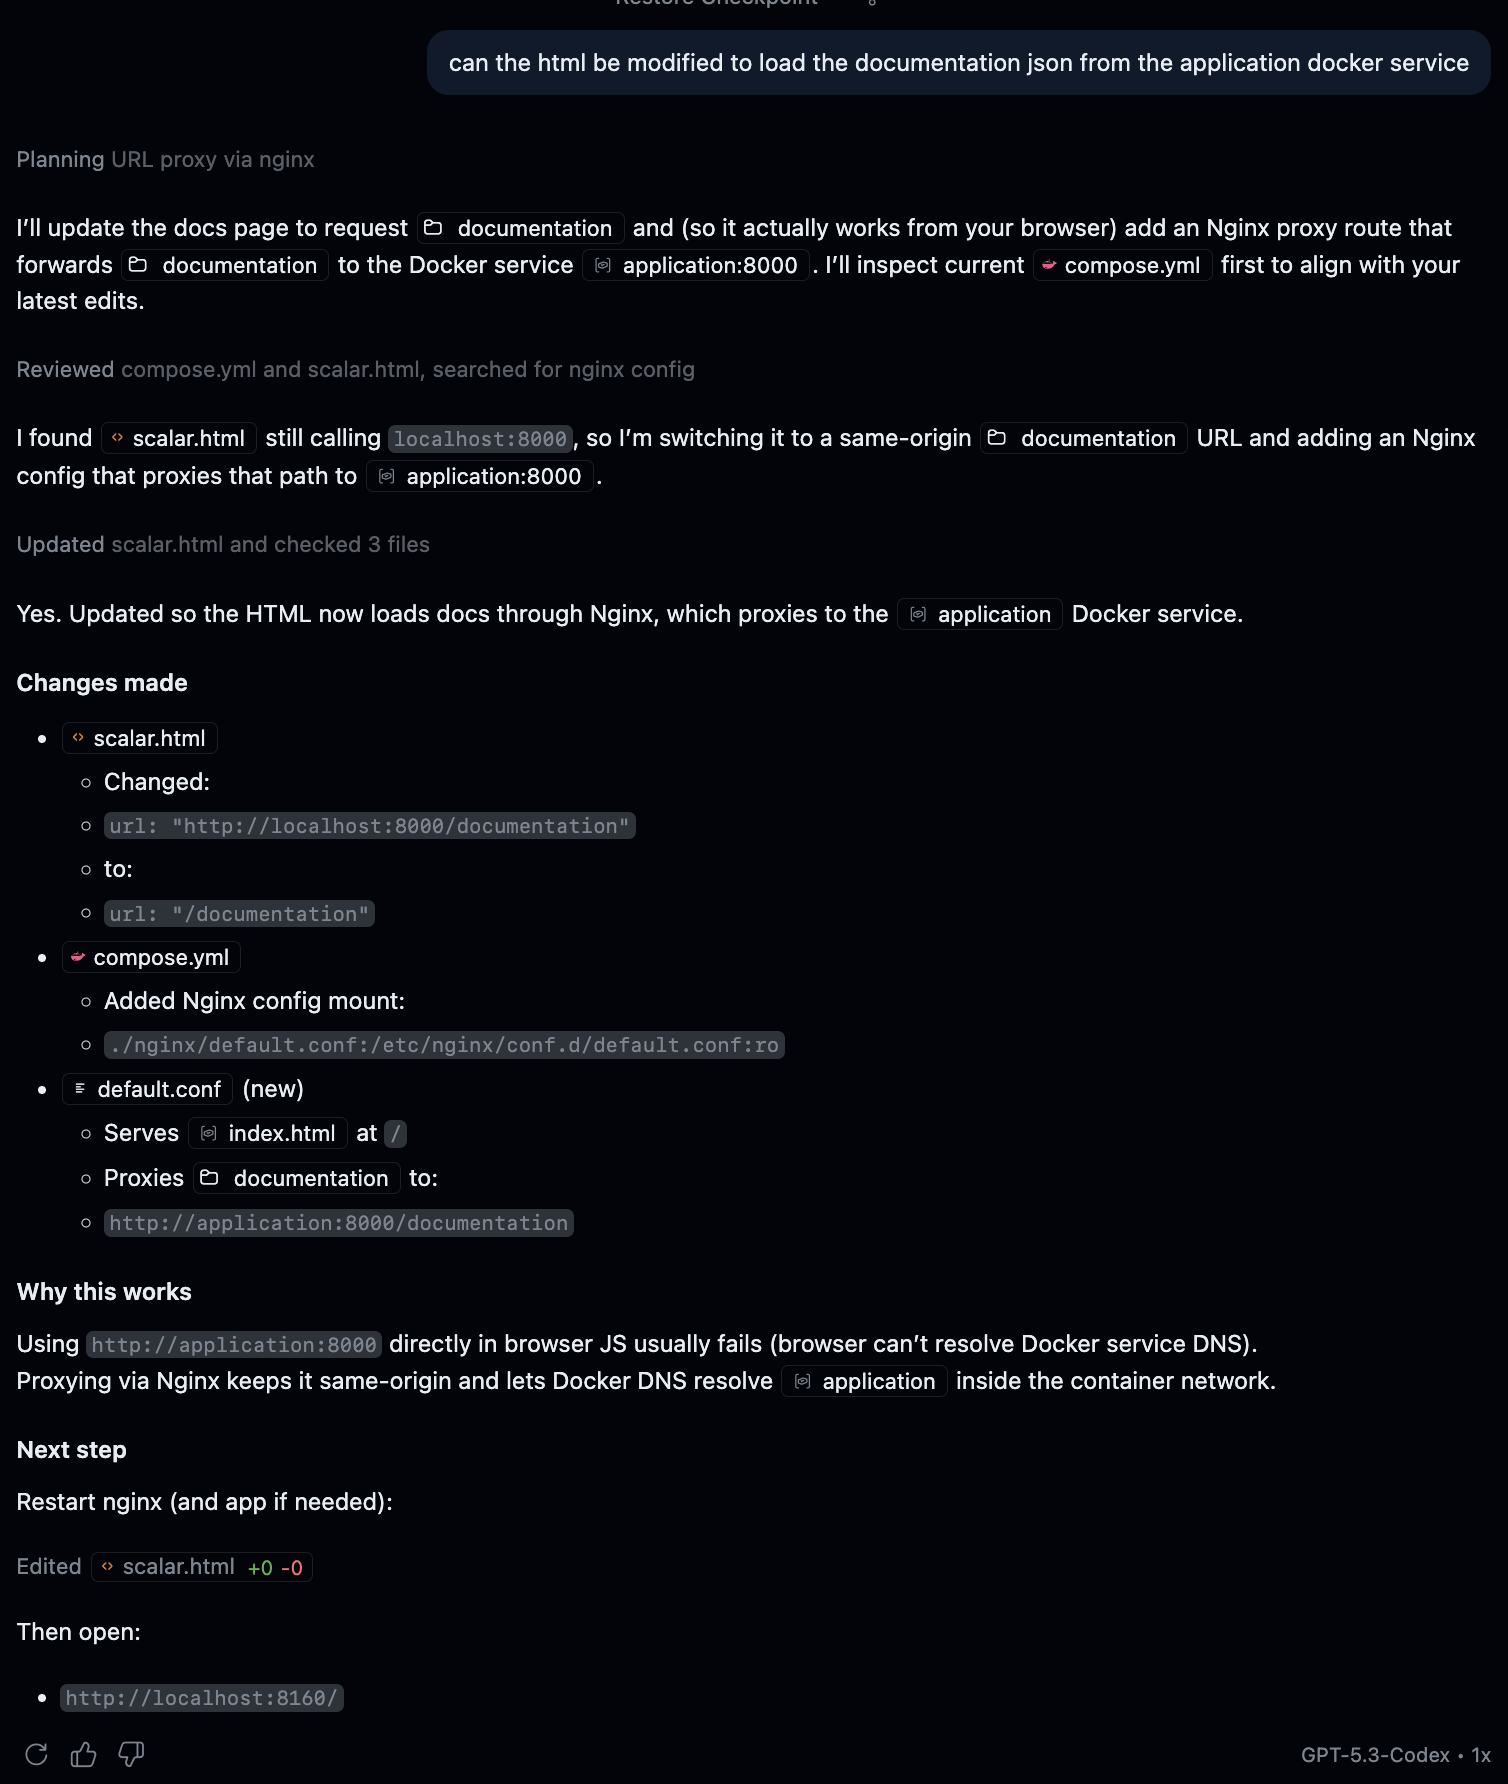
\includegraphics[width=0.6\linewidth]{ai-03.png}
\end{figure}

\begin{figure}[htbp]
  \centering
  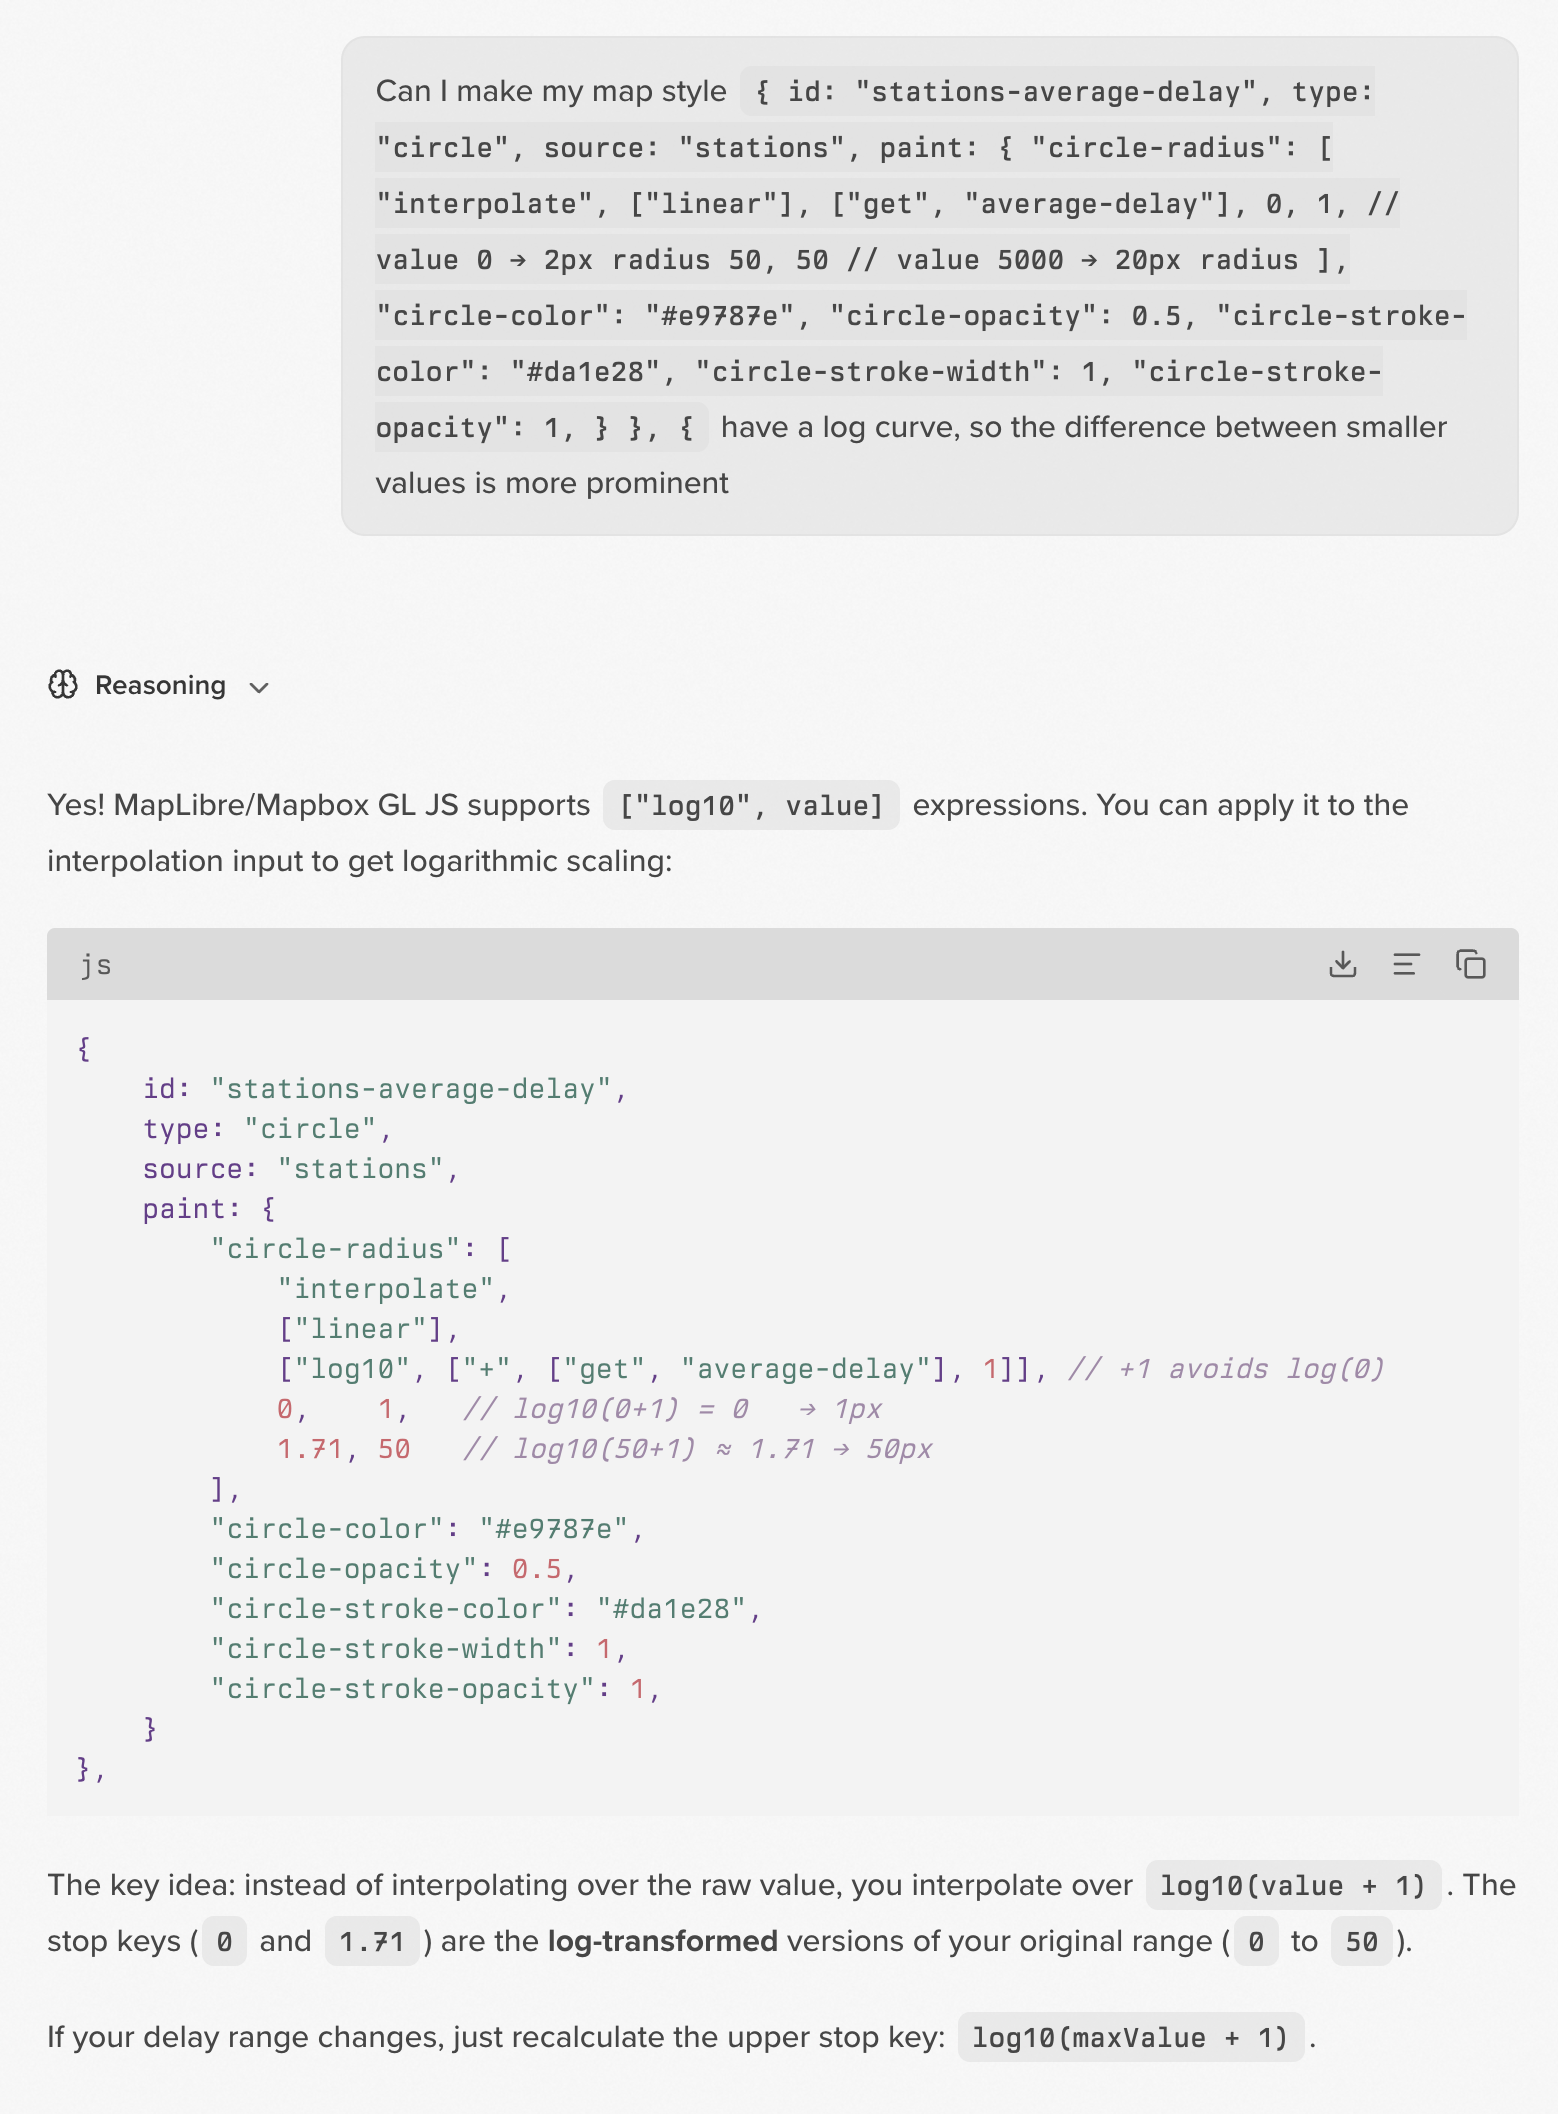
\includegraphics[width=0.6\linewidth]{ai-04.png}
\end{figure}

\end{document}